\section{E5: where do the mislabelled images go?}
\label{sec:e5}
The double-descent peak is driven by label noise, so we followed the 400 mislabelled images (20\% of $n=2000$) through trees below, at and above the interpolation point (same setup as E2; depth 2 with widths 4 to 1024, and depth 4 with widths 1 to 64). Three questions:
\begin{enumerate}
\item \emph{Do the routers isolate them?} Before running this, we expected the tree to \emph{quarantine} mislabelled images in a few small leaves, leaving the other leaves clean. We measured each leaf's share of mislabelled images under hard routing.
\item \emph{Do the routers bend to the wrong label?} For each class we know which leaves its correctly labelled images go to. A mislabelled image is \emph{label-routed} if its leaf is more typical of its (wrong) given label than of its true class. As a control, the same test is applied to clean images with a random fake label.
\item \emph{How far does the damage spread?} For each test image we find its nearest training image (in the 64-dimensional feature space). When that neighbour is mislabelled, how often does the tree predict the neighbour's wrong label, and how much higher is the test error there than near clean neighbours?
\end{enumerate}

\begin{table}[!htbp]
\centering\footnotesize
\begin{tabular}{rrrrrrrr}
\toprule
depth & width & params & test err & copies noisy NN label & err, NN noisy & err, NN clean & label-routed (control) \\
\midrule
2 & 4 & 2.0k & 46.9 & 8.5 & 50.7 & 46.1 & 42.0 (30.7) \\
2 & 16 & 5.6k & 50.5 & 9.6 & 55.0 & 49.5 & 53.7 (39.2) \\
2 & 64 & 20k & 66.9 & 14.6 & 73.8 & 65.2 & 47.0 (40.9) \\
2 & 256 & 78k & 55.2 & 15.9 & 63.8 & 53.2 & 47.3 (41.7) \\
2 & 1024 & 308k & 50.5 & 16.3 & 59.0 & 48.5 & 43.0 (43.6) \\
4 & 1 & 5.3k & 61.1 & 10.8 & 66.3 & 59.9 & 52.5 (29.7) \\
4 & 4 & 8.9k & 61.2 & 11.9 & 64.6 & 60.4 & 42.5 (32.4) \\
4 & 16 & 23k & 64.8 & 13.2 & 69.0 & 63.8 & 46.5 (33.5) \\
4 & 64 & 81k & 52.8 & 15.0 & 59.1 & 51.4 & 48.2 (36.2) \\
\bottomrule
\end{tabular}

\caption{E5 on CIFAR-10, 20\% noise. ``copies noisy NN label'': share of test images whose nearest training image is mislabelled and which receive that wrong label. ``err, NN noisy/clean'': test error on test images whose nearest training image is mislabelled / correctly labelled (19\% / 81\% of the test set). Label-routed: share of mislabelled training images whose leaf is more typical of the wrong label; the control is the same statistic for clean images with a random fake label.}
\label{tab:e5}
\end{table}

\begin{figure}[!htbp]
\centering
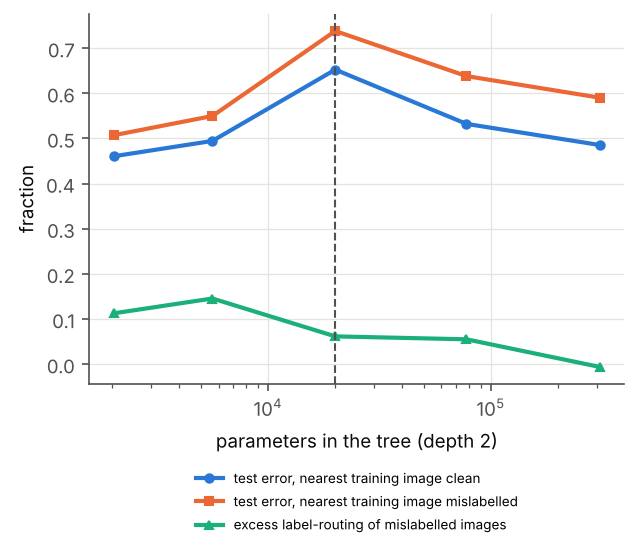
\includegraphics[width=0.55\linewidth]{e5_noise.png}
\caption{E5, depth-2 trees, 20\% noise. Dashed: the interpolation point. Excess label-routing is the label-routed share minus its control.}
\label{fig:e5}
\end{figure}

\paragraph{No quarantine.} The hypothesis was wrong. No leaf in any tree has twice the overall noise rate. Per-leaf noise rates lie between 14\% and 31\% in the depth-4 tree with width 64; the spread is widest in the smallest tree (depth 4, one hidden unit per leaf), whose two smallest leaves (16 and 19 images) have noise rates near 38\%. Mislabelled images are spread across all leaves, and each leaf memorises its own share.

\paragraph{Small leaves make the routers memorise.} Mislabelled images are label-routed more often than the control in every tree except the largest (Table~\ref{tab:e5}). The excess is largest when the leaves are too small to memorise anything themselves: 23 points for depth 4 with width 1 and 15 points for depth 2 with width 16. For depth 2 it falls to 6 points at and past the interpolation point and to zero at width 1024; with 16 leaves (depth 4) it stays at 10 to 13 points up to width 64. When the leaves can only draw simple boundaries, the routers absorb the wrong labels by steering mislabelled images to the leaves where images of the wrong class usually go. When the leaves are large, the leaves absorb them and the routing stays based on appearance.

\paragraph{The damage becomes local.} As the tree grows, it copies the wrong label of a mislabelled neighbour more often (8.5\% at width 4, 16.3\% at width 1024), and the error gap between test images near mislabelled and near clean training images widens from 4.6 to 10.5 points. Yet test error near \emph{clean} training images falls from 65.2\% at the interpolation point to 48.5\% at width 1024. The second descent therefore comes from test images away from the mislabelled ones. This is consistent with the large tree fitting each wrong label locally and staying smooth elsewhere, while the tree at the interpolation point distorts its function over a wider region to fit them. This matches the ``spiked-smooth'' picture of interpolating classifiers \cite{wyner2017}, and the tree adds a detail to it: which part of the tree does the fitting (routers or leaves) depends on leaf size.
